\documentclass{report}
\usepackage[a4paper,total={7in,10in}]{geometry}

\usepackage{amsmath}
\usepackage{amssymb}
\usepackage{enumitem}
\usepackage{tikz, pgfplots}
\usepackage{multicol}
\usepackage{setspace}
\usepackage{graphicx}
\usetikzlibrary{arrows}

\setcounter{chapter}{10}
\setcounter{section}{2}

\newcommand{\sol}{\vspace{1em}\\\textbf{Sol.}}
\newcommand{\eos}{ \qquad \square}

\begin{document}
\section*{Exercise 5c}

\onehalfspacing
\begin{enumerate}[leftmargin=*]
    \item Find the standard form of the equation of the ellipse that satisfies the given
          conditions:
          \begin{enumerate}
              \item Passes through point $P(-2\sqrt{2}, 0)$, $Q(0, \sqrt{5})$; \sol{}

                    Point $P$ is on the $x$-axis, while point $Q$ is on the $y$-axis.

                    $|OP| = 2\sqrt{2}$, $|OQ| = \sqrt{5}$,

                    $\because$ $|OP| > |OQ|$,

                    $\therefore$ The major axis is along the $x$-axis.

                    $\therefore$ The equation of the ellipse is of the form
                    \begin{align*}
                        \frac{x^2}{a^2} + \frac{y^2}{b^2} = 1
                    \end{align*}

                    Substituting the coordinates of $P$ and $Q$ into the equation, we get
                    \begin{align*}
                        \frac{(-2\sqrt{2})^2}{a^2} + \frac{0^2}{b^2} & = 1 \\
                        \frac{0^2}{a^2} + \frac{(\sqrt{5})^2}{b^2}   & = 1
                    \end{align*}
                    Simplifying, we get
                    \begin{align*}
                        \frac{8}{a^2} & = 1 \\
                        \frac{5}{b^2} & = 1
                    \end{align*}
                    Solving for $a$ and $b$, we get
                    \begin{align*}
                        a^2 & = 8 \\
                        b^2 & = 5
                    \end{align*}
                    $\therefore$ The standard form of the equation of the ellipse is
                    \begin{align*}
                        \frac{x^2}{8} + \frac{y^2}{5} = 1 \eos
                    \end{align*}
                    \vspace{1em}
                    \begin{center}
                        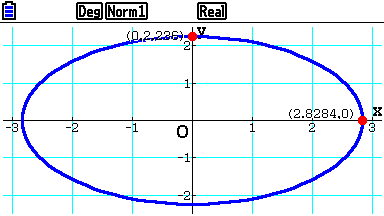
\includegraphics[scale=0.7]{./assets/ex5c1a.png}
                    \end{center}

                    \newpage
              \item Coordinates of its foci are $(-2\sqrt{3}, 0)$ and $(2\sqrt{3}, 0)$, and it
                    passes through the point $P(\sqrt{5}, -\sqrt{6})$;

                    The foci are on the $x$-axis, therefore let the equation of the ellipse be of
                    the form
                    \begin{align*}
                        \frac{x^2}{a^2} + \frac{y^2}{b^2} = 1
                    \end{align*}
                    From the coordinates of the foci, we have
                    $ae = 2\sqrt{3}$, $a^2e^2 = 12$,
                    \begin{align*}
                        \therefore\ b^2 & = a^2 - a^2e^2          \\
                                        & = a^2 - 12\ \cdots\ (1)
                    \end{align*}
                    Substituting the coordinates of $P$ into the equation $\dfrac{x^2}{a^2} + \dfrac{y^2}{b^2} = 1$, we get
                    \begin{align*}
                        \frac{(\sqrt{5})^2}{a^2} + \frac{(-\sqrt{6})^2}{b^2} & = 1 \\
                        \frac{5}{a^2} + \frac{6}{b^2}                        & = 1
                    \end{align*}
                    Substituting $(1)$ into the equation, we get
                    \begin{align*}
                        \frac{5}{a^2} + \frac{6}{a^2 - 12} & = 1                                           \\
                        5(a^2 - 12) + 6a^2                 & = a^2(a^2 - 12)                               \\
                        5a^2 - 60 + 6a^2                   & = a^4 - 12a^2                                 \\
                        a^4 - 23a^2 + 60                   & = 0                                           \\
                        (a^2 - 20)(a^2 - 3)                & = 0                                           \\
                        a^2 = 20\                          & \text{or}\ a^2 = 3\ (\text{rejected, } b > 0)
                    \end{align*}
                    When $a^2 = 20$, $b^2 = 20 - 12 = 8$.
                    $\therefore$ The standard form of the equation of the ellipse is
                    \begin{align*}
                        \frac{x^2}{20} + \frac{y^2}{8} = 1 \eos
                    \end{align*}
                    \vspace{1em}
                    \begin{center}
                        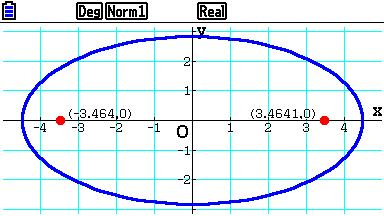
\includegraphics[scale=0.7]{./assets/ex5c1b.png}
                    \end{center}

                    \newpage
              \item Equations of its directrices are $y \pm \dfrac{25}{3} = 0$, and it passes
                    through the point $(4, 0)$; \sol{}

                    The directrices are perpendicular to the $y$-axis, therefore let the equation
                    of the ellipse be of the form
                    \begin{align*}
                        \frac{x^2}{b^2} + \frac{y^2}{a^2} = 1
                    \end{align*}
                    From the equation of the directrices, we have
                    $\dfrac{a}{e} = \dfrac{25}{3}$, $\dfrac{a^2}{e^2} = \dfrac{625}{9}$, $e^2 = \dfrac{9}{625}a^2$,
                    \begin{align*}
                        \therefore\ b^2 & = a^2 - a^2e^2                        \\
                                        & = a^2 - \frac{9}{625}a^4\ \cdots\ (1)
                    \end{align*}
                    Substituting the point $(4, 0)$ into the equation $\dfrac{x^2}{b^2} + \dfrac{y^2}{a^2} = 1$, we get
                    \begin{align*}
                        \frac{(4)^2}{b^2} + \frac{0^2}{a^2} & = 1 \\
                        \frac{16}{b^2}                      & = 1
                    \end{align*}
                    Substituting $(1)$ into the equation, we get
                    \begin{align*}
                        \frac{16}{a^2 - \dfrac{9}{625}a^4} & = 1                            \\
                        16                                 & = a^2 - \frac{9}{625}a^4       \\
                        9a^4 - 625a^2 + 10000              & = 0                            \\
                        (9a^2 - 400)(a^2 - 25)             & = 0                            \\
                        a^2 = 25\                          & \text{or}\ a^2 = \frac{400}{9}
                    \end{align*}
                    When $a^2 = 25$, $b^2 = 25 - \dfrac{9}{625}(25)^2 = 25 - 9 = 16$.

                    When $a^2 = \dfrac{400}{9}$, $b^2 = \dfrac{400}{9} -
                        \dfrac{9}{625}\left(\dfrac{400}{9}\right)^2 = 16$.

                    $\therefore$ The standard form of the equations of the ellipse is
                    \begin{align*}
                        \frac{x^2}{16} + \frac{y^2}{25} = 1\qquad \text{ or } \qquad \frac{x^2}{16} + \frac{9y^2}{400} = 1 \eos
                    \end{align*}
          \end{enumerate}
\end{enumerate}
\end{document}